% Beamer slide template prepared by Tom Clark <tom.clark@op.ac.nz>
% Otago Polytechnic
% Dec 2012

\documentclass[10pt]{beamer}
\usetheme{Dunedin}
\usepackage{graphicx}
\usepackage{fancyvrb}

\newcommand\codeHighlight[1]{\textcolor[rgb]{1,0,0}{\textbf{#1}}}

\title{Observer Pattern}

\author[IN710]{Object Oriented System Design}
\institute[Otago Polytechnic]{
  Otago Polytechnic \\
  Dunedin, New Zealand \\
}
\date{}
\begin{document}

%----------- titlepage ----------------------------------------------%
\begin{frame}[plain]
  \titlepage
\end{frame}

\begin{frame}
	\frametitle{Problem: Bicycle dashboard}

	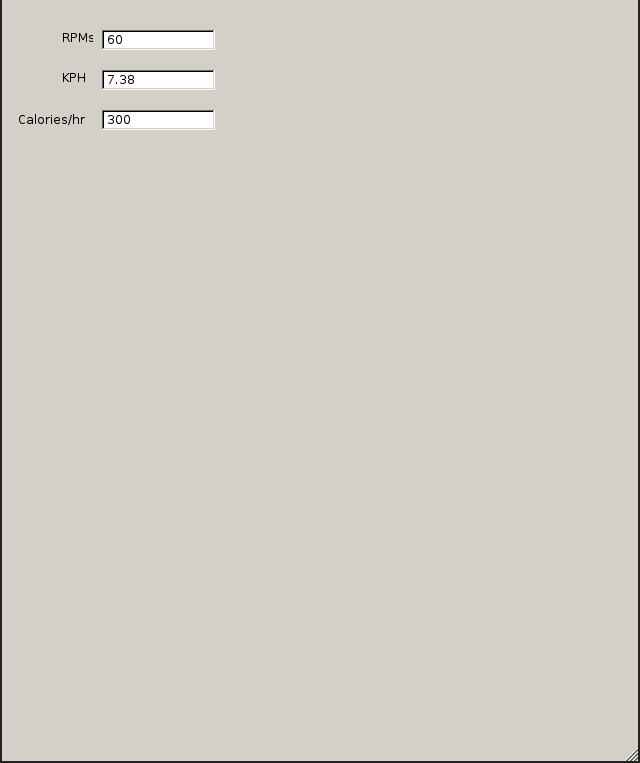
\includegraphics[scale=.5]{ss.png}
\end{frame}

\begin{frame}
	\frametitle{Problem: Bicycle dashboard}

	\begin{itemize}
		\item We will enter the RPMs.
		\item When the RPMs change, we update
			\begin{itemize}
				\item the speed
				\item the calories per hour
			\end{itemize}
	\end{itemize}
\end{frame}

\begin{frame}
	\frametitle{Solution: Subject/Observers}

	Classes involved:
	\begin{description}
		\item[Bicycle (\emph{subject})] keeps track of its RPMs
		\item[Speedometer (\emph{observer})] determines speed from RPMs
		\item[Calorie meter (\emph{observer})] determines calories/hour from RPMs
	\end{description}
\end{frame}

\begin{frame}
	\frametitle{Implementing subject/observer}

	\begin{itemize}
		\item The \emph{subject} maintains a list of its observers.
		\item It \emph{notifies} the observers when an event occurs.
		\item The \emph{observers} register themselves with their subject.
		\item They provide an \texttt{update} method to respond to 
			notifications from the subject.
	\end{itemize}
\end{frame}

\begin{frame}[fragile]
	\frametitle{Subject code}

	\begin{verbatim}

     class Bicyle:

        def add_observer(self, o):
            # append o to list of observers

        def remove_observer(self, o):
            # remove o from list

        def notify_observers(self):
            # iterate over observer list and call each
            # of their update methods

	    \end{verbatim}
\end{frame}

\begin{frame}[fragile]
	\frametitle{Observer code}

	\begin{verbatim}

    class Speedometer:
        
        def __init__(self, subject):
            # save reference to subject
            # call subject's add_observer method, 
            # passing in self

        def update(self, rpms):
            # subject will call this when rpms change


	    \end{verbatim}
\end{frame}

\begin{frame}
	\frametitle{Practical exercise}

	\begin{itemize}
		\item Write the needed bicycle dashboard classes,
			\texttt{Bicycle}, \texttt{Speedometer},
			\texttt{CalorieMeter} using an
			observer pattern.
		\item Use a wheel circumference of 205 cm for speed calculations.
		\item You can test these in your interactive Python
			interpreter session, but you may want to 
			build a gui for this.
		\item See \url{http://pythonforengineers.com/your-first-gui-app-with-python-and-pyqt/}
	\end{itemize}
\end{frame}


\end{document}
